\chapter{Análisis de tecnologías}
\label{sec:analisis_tecnologias}

\section[Python]{Python}

Python es un lenguaje de programación de alto nivel, de propósito general e interpretado. Es un lenguaje open-source y por ende, el código fuente se puede obtener bajo la licencia GNU General Public License (GPL). Python permite programar de forma fácil y clara, tanto como para pequeña y gran escala proporcionando de varias construcciones. Su filosofia de diseño se enfatiza en la legibilidad, usando espacios en blanco. Mas importante, Python incorpora los paradigmas de programación orientada a objetos, imperativo, funcional y procedural con una biblioteca estándar muy enriquecida.

\subsection[Es interpretado]{Es interpretado}

Python es procesado en tiempo de ejecución por el intérprete, no requiere compilación el programa entero antes de ser ejecutado. El intérprete directamente ejecuta el programa, linea por linea traduciendo cada declaración en una secuencia de subrutinas y luego a código máquina. Esto hace que sea más flexible que otros lenguajes de programación proporcionando un programa ejecutable más pequeño.

\subsection[Es orientado a objetos]{Es orientado a objetos}

Python es un lenguaje de programación multi paradigma. Por esto, soporta el estilo orientado a objetos, las reglas y técnicas de programación que encapsulan código dentro de los objetos. Además, todo el código escrito en el fuente de Python está en forma de objetos y clases.

\subsection[Es portable]{Es portable}

Python tiene la capacidad de correr en una gran cantidad de plataformas de hardware con la misma interfáz. Corre perfectamente en todos los sistemas operativos como Windows, Linux, UNIX, Amigo, MacOs, etc.

\subsection[Es extensible]{Es extensible}

Python es tán versátil y flexible que permite a los programadores agregar módulos, de bajo o alto nivel, que ya existan o crear sus propios módulos para agregarlos al intérprete. Estos módulos y paquetes de herramientas permiten a los programadores desarrollar de una forma portable y multiplataforma, que les permite crear y personalizar sus programas, aplicaciones, o herramientas de software para ser mas eficientes. 

\subsection[Es de scripting]{Es de scripting}
Python puede ser utilizado como un lenguaje de scripting, tanto Batch como Interactive. Además, sigue reglas de alcance simples, por lo tanto, se puede hacer un tipado dinámico flexible. Además, al ser un lenguaje de script, permite un fácil acceso a otros programas. Se puede compilar en código de bytes para construir aplicaciones grandes.

\subsection[Es web]{Es web}
Python ofrece una variedad de elecciones para el desarrollo de aplicaciones web, y esto se debe a su escalabilidad. La liberaria estándar de Python incorpora muchos protocolos para el desarrollo web, como HTML, XML, JSON, procesamiento de emails. También provee las bases para FTP, IMAP, y otros protocolos de internet.

Siendo tan flexible, provee un fácil uso de la interfáz socket, además de libererias como Requests (un cliente HTTP), BeatifulSoup (parser HTML), Feedparser (parser RSS/Atom), entre otras. Además de las librerias mencionadas, tiene varios frameworks web como Django, Flask, Pyramid, etc. 


\section[Django]{Django}

Django es un framework de desarrollo web de código abierto, que respeta el patrón de diseño MVC (Modelo Vista Controlador). Fue diseñado como un framework del lado del servidor, que opera con bases de datos relacionales. Sin embargo, a lo largo de los años se fue adaptando a las necesidades y puede operar con bases de datos no relacionales (a través de paquetes de terceros).

El contenido en los proyectos de Django trabaja en 3 grandes bloques: urls, templates y apps. Se definen de forma separada y se conectan para cumplir con la entrega de contenido, que es parte de los principios de arquitectura poco acoplada que promueve Django.
Las URLs definen puntos de entrada de acceso al contenido. Los templates definen los puntos de salida que dan forma al contenido final. En el medio, las apps sirven como *middleware* entre las urls y los templates, agregando contenido desde una base de datos o la interacción de un usuario. 
Para servir código estático, solo se necesitan crear y configurar urls y templates. Para contenido dinámico, se necesitan crear y configurar apps.

\begin{figure}[h!]
  \centering
    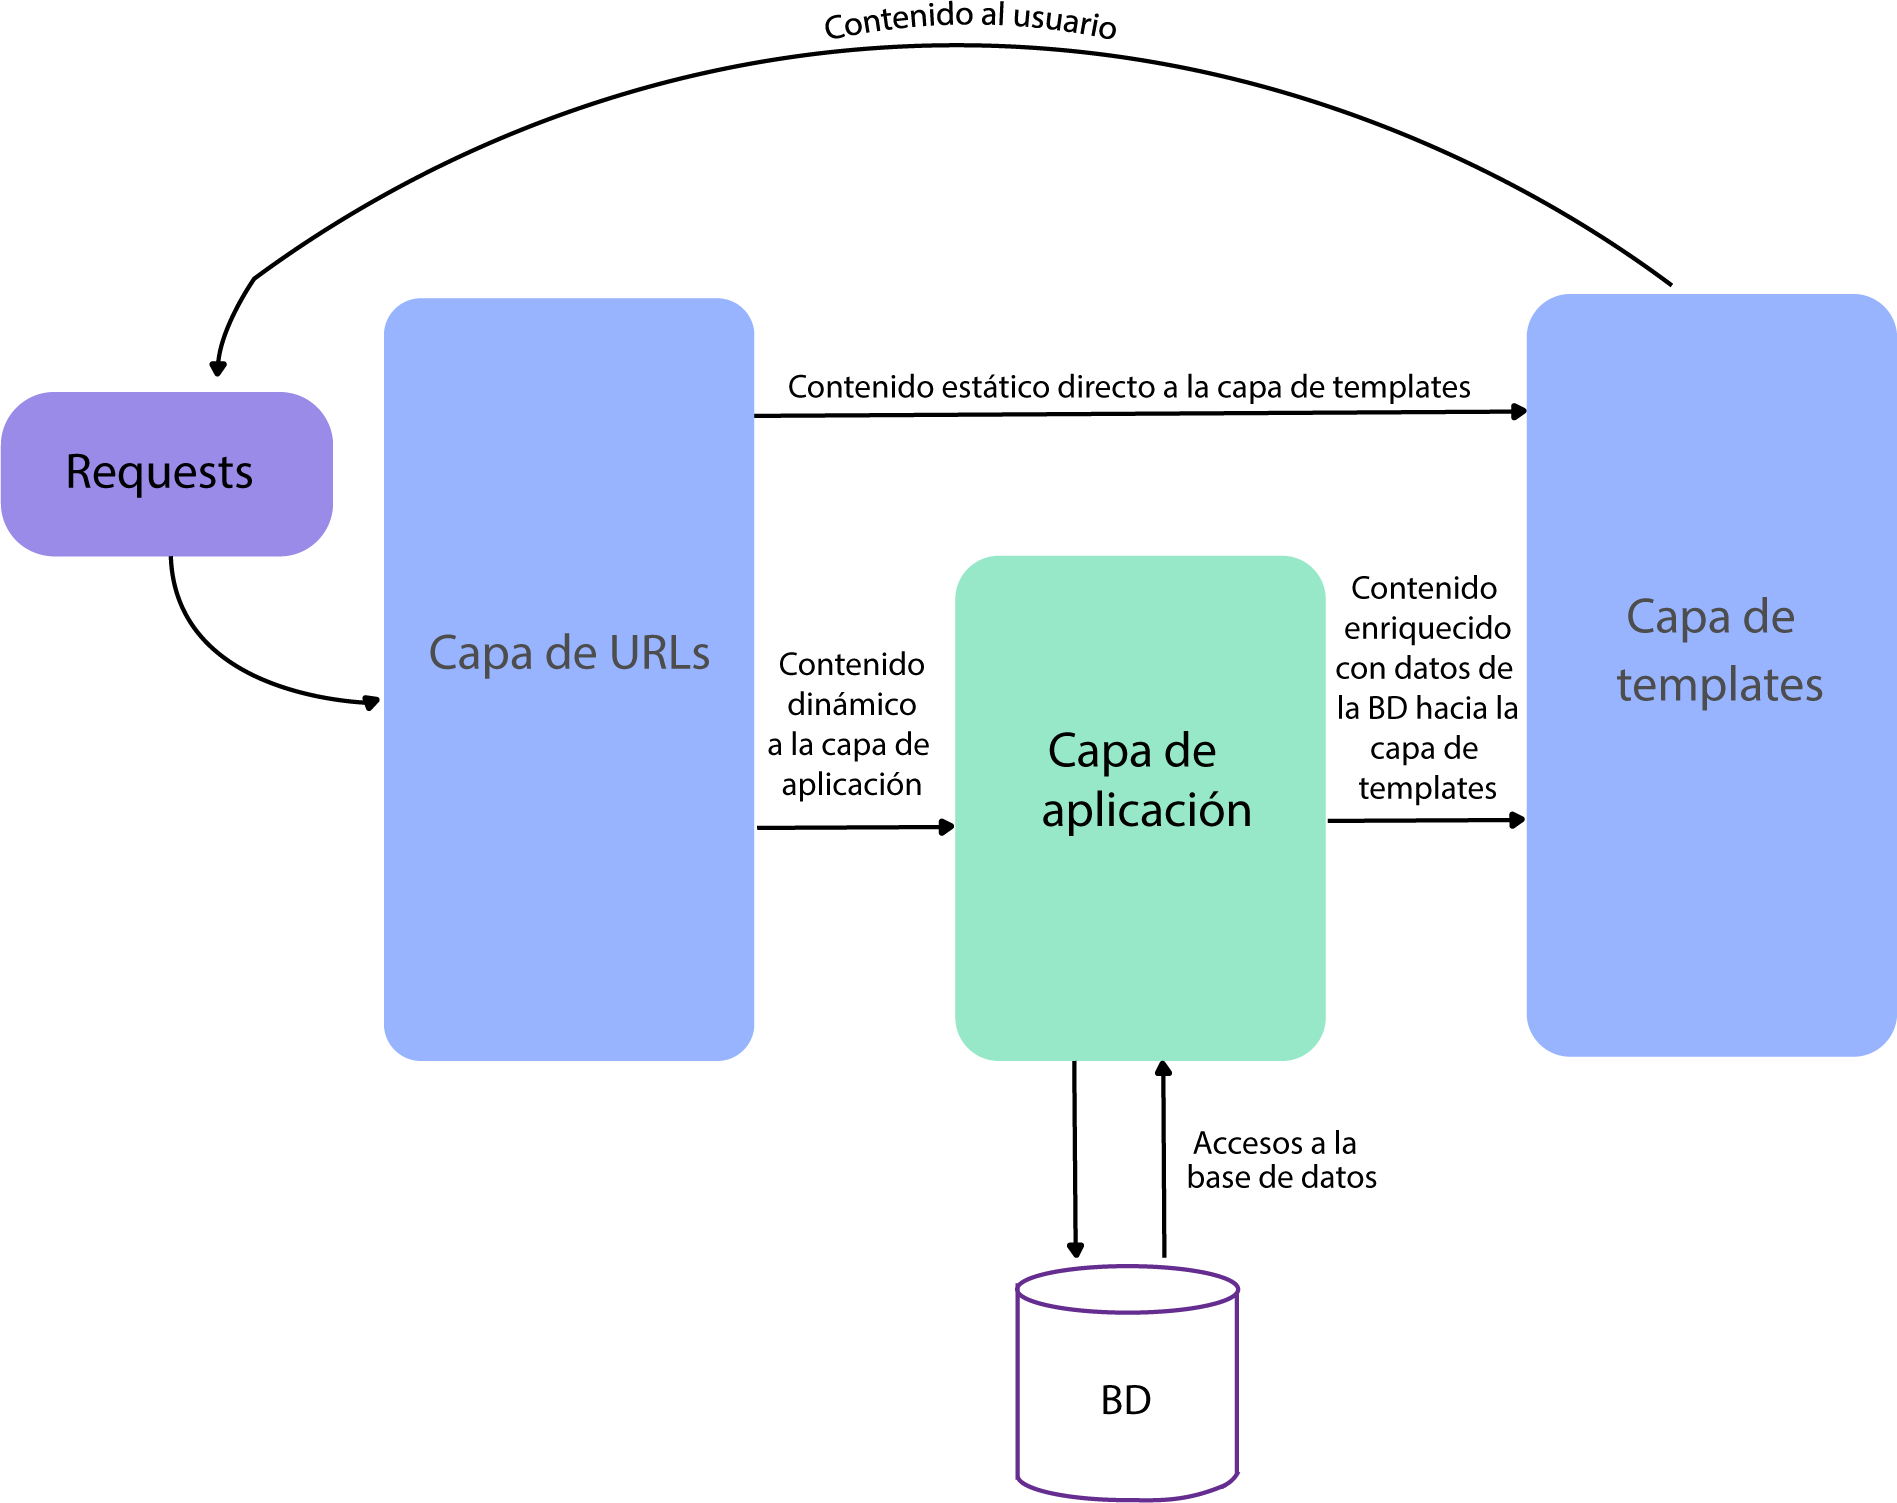
\includegraphics[scale=0.9]{images/django.png}
  \captionof{figure}{Flujo de trabajo de Django}
  \label{fig:django}
\end{figure}

Como se puede ver en la figura, hay dos flujos de información. Uno para enviar información estática, y el otro para enviar información dinámica.

\section[Flask]{Flask}

Flask es un framework chico para casi cualquier estándar. Suficientemente chico para que sea llamado "micro-framework"\cite{Fsck}. Pero ser chico no significa que hace menos que otros frameworks, sino que fue diseñado para ser extensible desde los cimientos. Provee un núcleo sólido con los servicios básicos, mientras el resto puede ser provisto por extensiones. El hecho de que permita elegir y poner la extensión que se desee, hace que se termine usando un framework que no tiene funcionalidades de más y sirve para exactamente lo que se necesite.
Flask tiene tres dependencias principales: rutas, debugging y WSGI (Web Server Gateway Interface, provisto por Werkzeug); los templates son provistos por Jinja2, y la interacción por línea de comandos viene de Click. Estas dependencias fueron escritas por Armin Ronacher, el autor de Flask.
Flask no dispone de acceso nativo a bases de datos, validar formularios web, autenticación, u otras tareas de alto nivel. Sólo se pueden usar a través de extensiones. Como desarrollador, se puede decidir integrar la que se desee o escribir una propia. Esto va en contraste con grandes frameworks, ya que es complejo o imposible cambiar estas funcionalidades.

\section[Python en Data Science]{Python en Data Science}

La comunidad de la ciencia de datos está cambiando de R a Python, ya que provee a los científicos una gran cantidad de funcionalidades y les permite crear sus propias funcionalidades para realizar cálculos muy complejos. Además, les permite generar varios tipos de reportes de análisis, histogramas, grafos, y mucho más.
Existen muchos módulos de Data Science, entre ellos numpy, Pandas, etc.

\subsection[Numpy]{Numpy}

NumPy, abreviatura de Numerical Python, viene siendo hace mucho tiempo una parte fundamental para la computación numérica. Provee estructuras de datos, algoritmos y liberías necesarias para la mayoría de las aplicaciónes científicas que involucran datos numéricos en Python. NumPy contiene entre otras cosas:
\begin{outline}
    \1 ndarray: Un array multidimensional rápido y eficiente.
    \1 Funciones para realizar cálculos basados en elementos con matrices u operaciones matemáticas entre matrices
    \1 Herramientas para leer y escribir datasets al disco.
    \1 Operaciones de álgebra lineal y generación de números aleatorios.
    \1 Una API en C muy madura que permite a las extensiones de Python acceder a las estructuras de datos de NumPy
\end{outline}
Mas allá de las capacidades de procesamiento de matrices que NumPy le agrega a Python, una de sus principales usos para análisis de datos es como contenedor para que los datos sean pasados entre algoritmos y librerías. Para datos numéricos, los arrays de NumPy son más eficientes para guardar y manipular los datos que cualquier otrá librería de Python.


\subsection[Pandas]{Pandas}

Pandas provee estructuras de datos de alto nivel y funciones diseñadas para trabajar con datos estructurados o tabulados de forma rápida, fácil y expresiva. Desde su salida en 2010 fue ayudando a Python a crear un entorno de análisis de datos poderoso y productivo. Los objetos principales de pandas son: 
\begin{outline}
    \1 DataFrame: una estructura de datos tabular, orientada a columnas, con etiquetas por columna y fila.
    \1 Series: un array etiquetado de una dimensión.
\end{outline}

Pandas mezcla la alta performance de las ideas computacionales sobre arrays de Numpy, con las capacidades flexibles de la manipulación de datos de las hojas de cálculos y las bases de datos relacionales (como SQL). Además, provee funcionalidades de indexación sofisticadas para que resulte fácil la remodelación, corte, agregación y selección de subconjunto de datos.

Pandas surgió en 2008 para cumplir con ciertos requerimientos que ninguna otra herramienta podía satisfacer:

\begin{outline}
    \1 Estructuras de datos con ejes etiquetados, y que soporte alineación de datos automática o explícita. Esto previene errores comunes resultantes de trabajar con datos provenientes de distintas fuentes.
    \1 Series de tiempo integradas.
    \1 Estructura de datos que pueda manejar series de tiempo y otros datos a la vez.
    \1 Operaciones aritméticas y reducciones que preserven los metadatos.
    \1 Manejo de datos faltantes de forma flexible.
    \1 Unión y otras operaciones relacionales encontradas en bases de datos.
\end{outline}

\section[React]{React}

React es una librería de Javascript que tiene como propósito simplificar el desarrollo de interfaces visuales.
Fue desarrollado por Facebook y lanzado al mundo en 2013.
Su objetivo principal es facilitar el razonamiento sobre las interfaces y su estado en cualquier momento, dividiendo la UI en una colección de componentes.

\subsection[Componente]{Componente}

Los componentes permiten separar la interfaz de usuario en piezas independientes, reutilizables y pensar en cada pieza de forma aislada.
Conceptualmente, los componentes son como las funciones de JavaScript. Aceptan entradas arbitrarias (llamadas “props”) y devuelven a React elementos que describen lo que debe aparecer en la pantalla.
Los componentes pueden referirse a otros componentes en su salida. Esto nos permite utilizar la misma abstracción de componente para cualquier nivel de detalle. Un botón, un cuadro de diálogo, un formulario, una pantalla: en aplicaciones de React, todos son expresados comúnmente como componentes.


\subsection[DOM Virtual]{Dom Virtual}

DOM (Document Object Model) es un arbol que representa una página, empezando con la etiqueta <html>, bajando por cada hijo llamado nodo.
Se guarda en la memoria del navegador y se vincula directamente con lo que se ve en una página. El DOM tiene una API, con la cual se puede acceder a él, acceder a cada nodo, filtrarlos, modificarlos.
React mantiene una copia de la representación del DOM al que llama DOM virtual.

Cada vez que el DOM cambia, el navegador tiene que realizar dos operaciones intensivas: repintar (cambios visuales o de contenido en un elemento que no afectan el diseño y el posicionamiento en relación con otros elementos) y reflujo (recalcular el diseño de una parte de la página, o el diseño completo de la página).
React usa DOM Virtual para ayudar al navegador a usar menos recursos cuando se necesita que haya cambios en la página.

React sólo cambia el DOM cuando el estado de un componente cambia explícitamente.
Cuando hay un cambio, React actualiza el DOM Virtual relativo al componente que necesita cambiar.
La clave está en que sólo actualiza el DOM una vez, asi el "repintado" y "reflujo" que tiene que realizar el navegador se hace sólo una vez.


\section[Microservicios]{Microservicios}

Los microservicios son servicios pequeños y autónomos que trabajan en conjunto. 
A medida que el código va creciendo cuando se agregan funcionalidades, se hace cada vez complejo saber dónde se tienen que hacer los cambios.
Las funcionalidades nuevas empiezan a quedar esparcidas por todo el código, haciendo que sea cada vez más dificil encontrar errores.

Los microservicios afrontan un acercamiento hacia la independencia de servicios. Enfocandose en la obviedad donde el código solo sirve para alguna funcionalidad. Y al mantener este servicio enfocado dentro de sus límites, se evita que crezca demasiado.

\subsection[Heterogeneidad Tecnológica]{Heterogeneidad Tecnológica}

Con un sistema compuesto de multiples servicios colaborando entre sí, podemos elegir usar diferentes tecnologías dentro de cada uno de éstos. Esto permite elegir la herramienta correcta para cada trabajo, en lugar de tener que elegir una opción que sirva un poco para todo, y puede terminar siendo perjudicial para el sistema.

Si una parte del sistema necesita mejorar su performance, podemos decidir cambiar de tecnología a una que resulte mejor para esa tarea en particular.

\begin{figure}[h!]
  \centering
    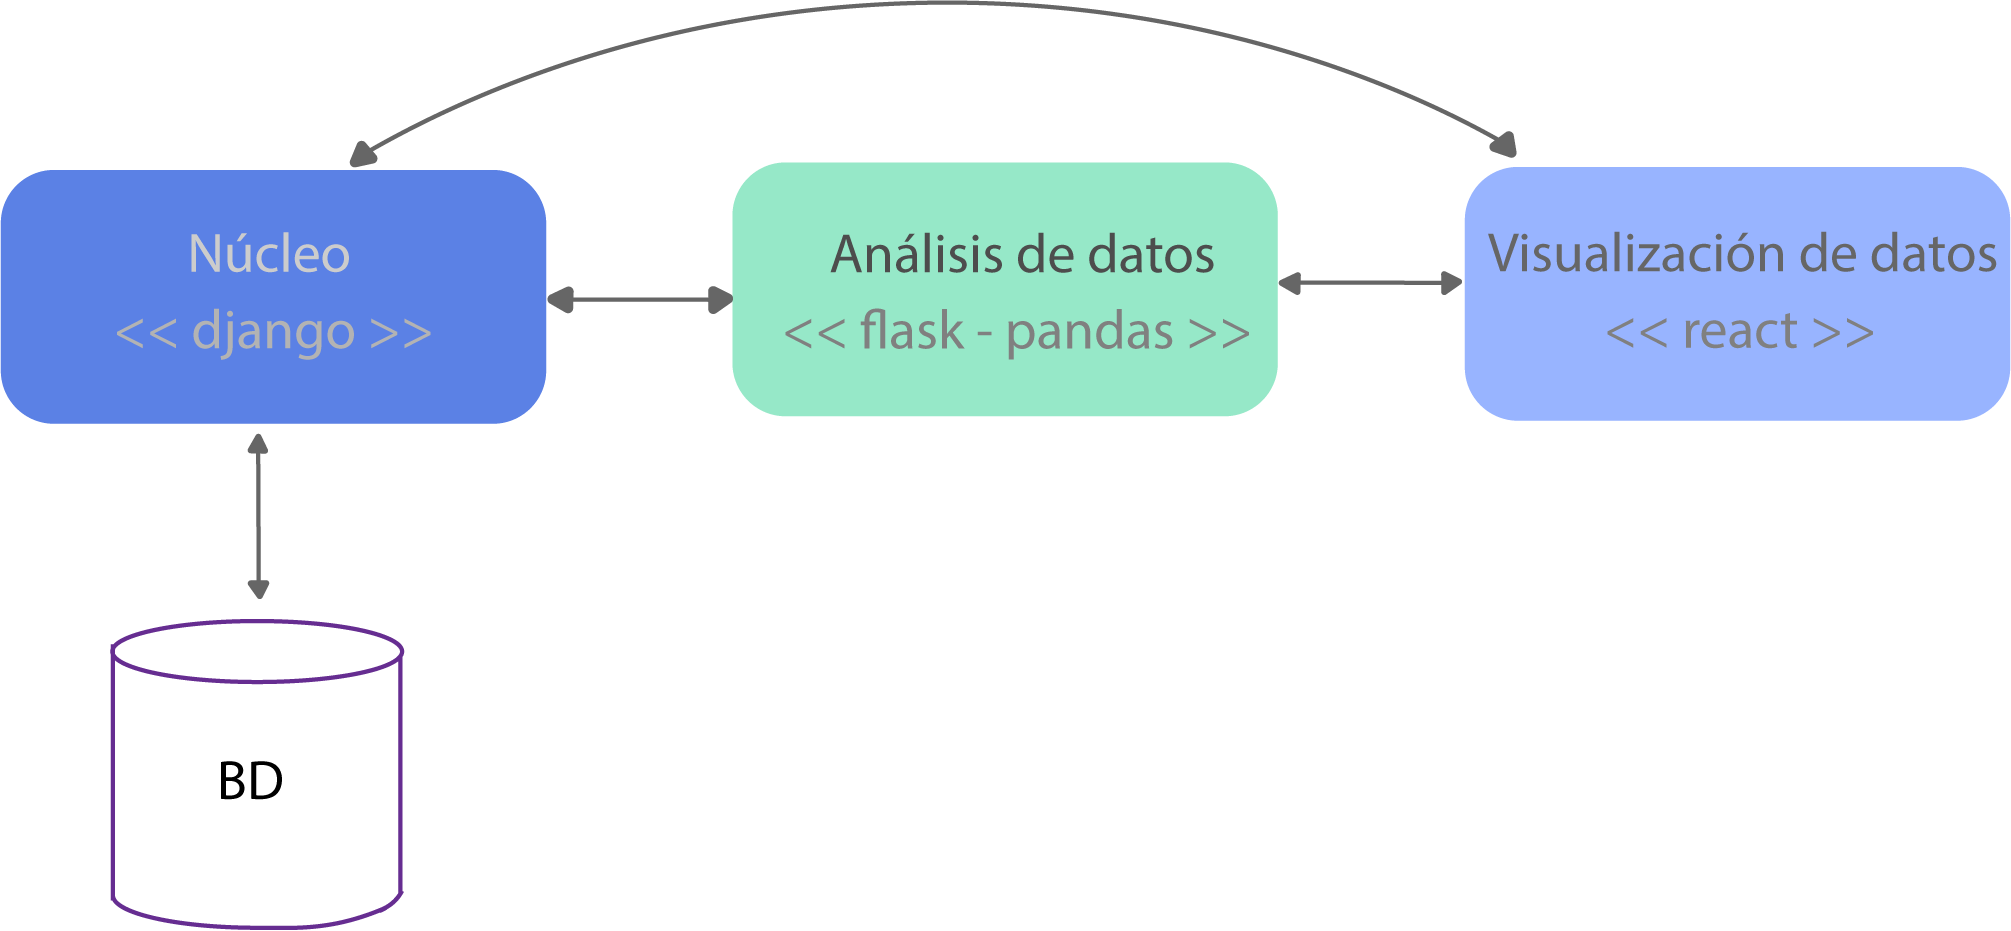
\includegraphics{images/heterogeneidad-tecnologica.png}
  \captionof{figure}{Microservicios: Homogeneidad Tecnológica}
  \label{fig:microht}
\end{figure}

\break

El gráfico muestra tres servicios distintos, un núcleo que usa Django, un servicio de análisis de datos, con Flask y Pandas, y un servicio de visualización de datos con React.

\subsection[Independencia]{Independencia}

En un sistema monolítico, cuando hay una falla todo el sistema se corrompe. Aunque se pueda mitigar usando varias instancias del mismo sistema, esto no es conveniente ya que a medida que el sistema va creciendo, tener varias instancias de un sistema grande necesitaría una mayor capacidad de procesamiento.
Desde la perspectiva de microservicios, cuando uno de los servicios tenga una falla y esa falla no genere un problema en cascada, se puede aislar el problema y así el resto de los servicios puede seguir funcionando. 

\subsection[Escalamiento]{Escalamiento}

En un sistema monolítico, todo se escala junto. Si sólo se necesitara que un servicio determinado tenga mas recursos, estaría dándole más recursos a todo el sistema.
En cambio, con microservicios, si en un determinado momento se necesita, por ejemplo, que el servicio de análisis de datos procese mas peticiones se podría escalar sólo ese servicio teniendo dos instancias (o más) de esa parte del sistema, dejando los otros módulos corriendo con hardware menos poderoso, acorde a sus necesidades.

\begin{figure}[h!]
  \centering
    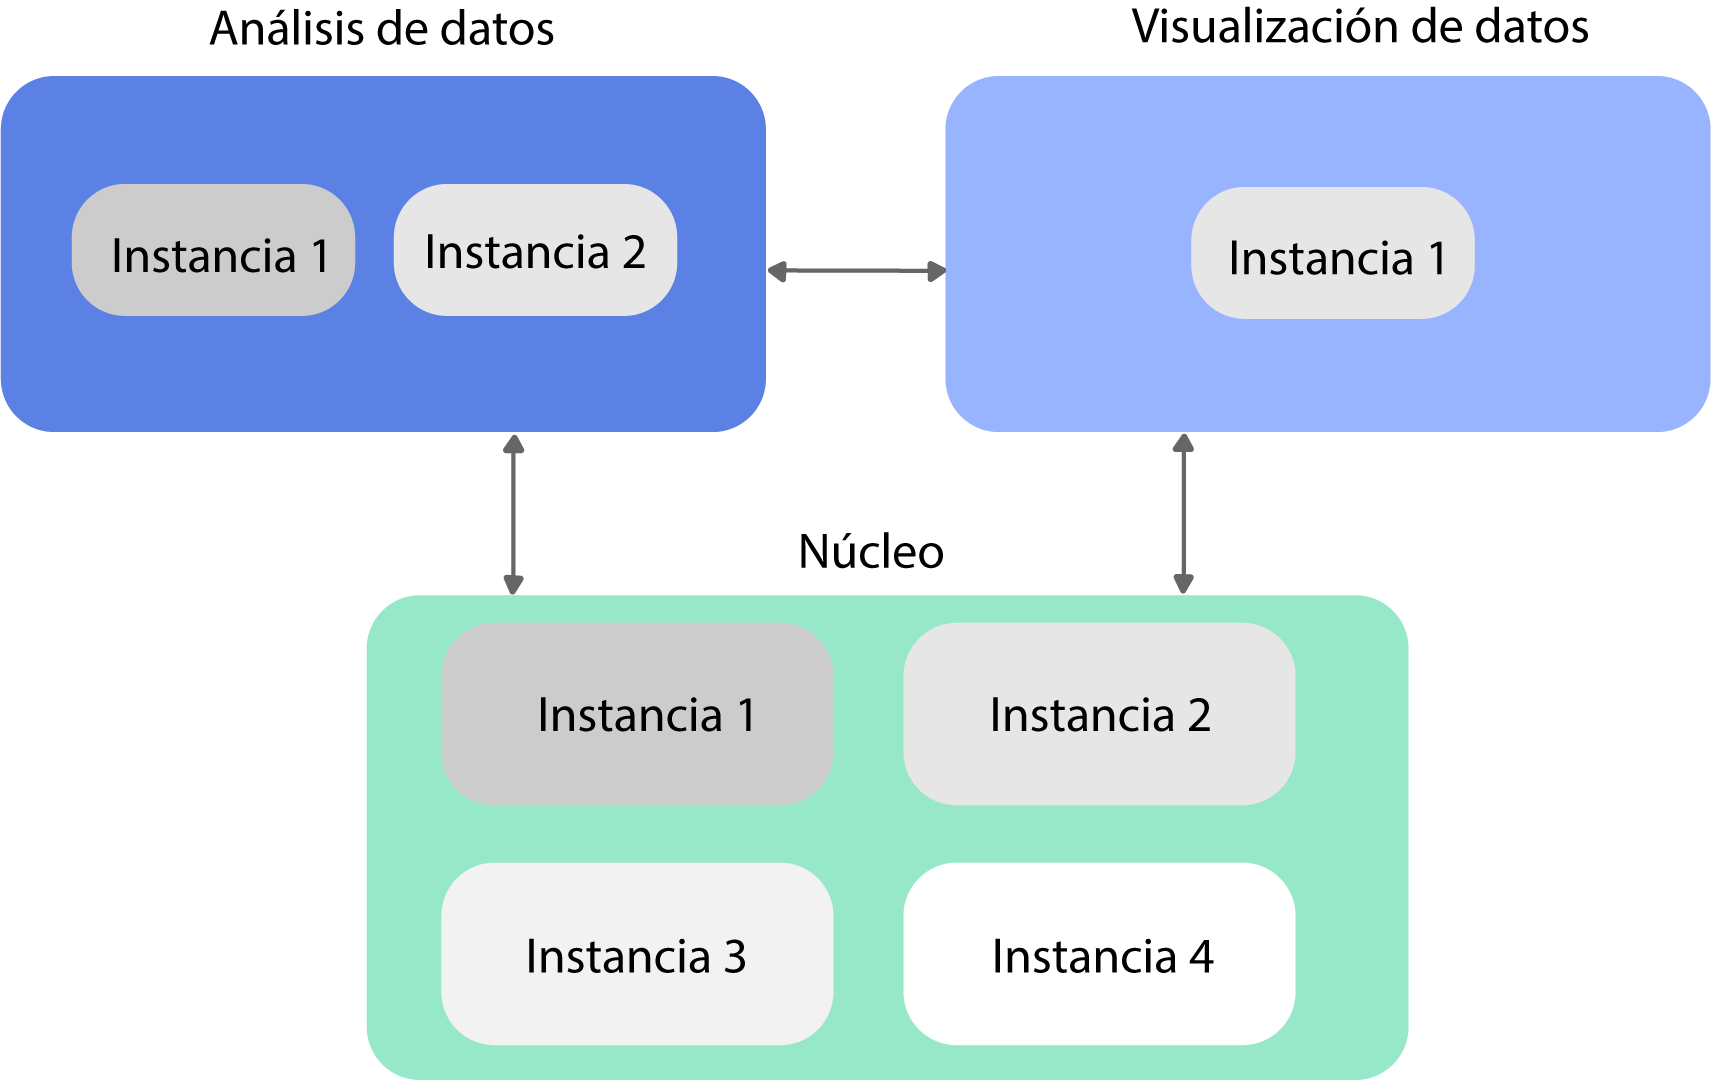
\includegraphics[scale=0.7]{images/escalamiento.png}
  \captionof{figure}{Microservicios: escalamiento}
  \label{fig:microescala}
\end{figure}

\subsection[Facilitar deploy]{Facilitar deploy}

Hacer un pequeño cambio en un sistema monolítico requeriría deployar toda la aplicación para hacer efectivo el cambio. Esto genera un gran impacto y un alto riesgo. 
Desde la perspectiva de los microservicios, el cambio que se hace sobre un servicio permite deployar sólo ese módulo, sin que los otros sepan que hubo una modificación. Además, el código es deployado mas rápido. 
De haber un problema en la actualización, se puede aislar a un sólo servicio, permitiendo retroceder a una versión anterior.

\subsection[Reemplazabilidad]{Reemplazabilidad}

El costo de reemplazar un servicio por una mejor implementación es más fácil de manejar cuando hay independencia. 
Si en un futuro se quisiera, por ejemplo, cambiar el módulo de encuestas, sólo haría falta reemplazar ese pequeño sistema sin tener que modificar el resto. Ni siquiera deberian enterarse del cambio.

>> Gráfico conceptual del nucleo y otras apps

\section[REST]{Rest}

REpresentational State Transfer (Transferencia de estado representacional, su traducción) es un estilo arquitectural inspirado en la Web. 
Una parte importante es el concepto de **recursos**. 
El servidor crea diferentes representaciones del recurso en un request. La forma en que es enviado esta desacoplado a cómo está guardado internamente. Cuando un cliente pide por un recurso, se le da una representación con la estructura de JSON.
A lo largo de los años, se desarrollaron muchos servicios basados en la arquitectura REST, que usa las funcionalidades provistas por la capa de aplicación del protocolo HTTP \cite{RestSoap} \cite{IETF}. Esto resultó en un incremento en el interés comparado al tradicional SOAP (Simple Object Access Protocol). Además, grandes compañías como Twitter o Amazon usan interfaces del tipo REST en sus servicios, lo cual se puede ver en la documentación de sus APIs (Application Programming Interface).
Mas allá de la tendencia, no hay estándares o guias de cómo desarrollar un servicio web RESTful. En lugar de esto, existen buenas prácticas.

\subsection[No versionado]{No versionado}

Versionar una API Web es una de las consideraciones más importantes a la hora de diseñar un servicio web, ya que la API representa el punto de acceso al servicio y oculta su implementación. Es por esto que una interfaz web nunca deberia ser desplegada sin un identificador de version \cite{WAPID}. Para versionar, existen diferentes acercamientos como incluirlo en la URI (Uniform Resource Identifier) del servicio web o usando el header HTTP para seleccionar la versión apropiada \cite{WAPID}. Pero el servicio web basado en REST no necesita ser versionado debido a hipermedia. Es por esto que los servicios web RESTful pueden ser comparados con los sitios web tradicionales, que pueden ser accedidos por todos los navegadores cuando se cambia el contenido del sitio. Asi que no sería necesario agregar información del lado del cliente.
Mas allá de esto, el uso de versionado genera un impacto negativo en los servicios web ya desplegados, ya que aumenta el esfuerzo por mantenerlos.


\subsection[Descripción de los recursos]{Descripción de los recursos}

La descripción de los recursos se relaciona con la usabilidad de los servicios web, ya que éstos son una representación del modelo. Para una correcta descripción, existen algunas buenas prácticas:
\begin{outline}
    \1 Deberían usarse sustantivos para los recursos \cite{WAPID}.
    \1 El nombre del recurso debería ser un nombre específico del dominio, para que la semántica pueda ser interpretada por cualquier usuario sin conocimientos adicionales \cite{WAPID}
    \1 Debería evitarse la mezcla del uso del plural y singular para garantizar coherencia \cite{WAPID}.
    \1 Debería usarse la convención de nombres de JavaScript, ya que el tipo JavaScript Object Notation (JSON) es el tipo de dato más usado para la comunicación entre el cliente y el servidor \cite{WAPID}.
\end{outline}
\subsection[Identificación de recursos]{Identificación de recursos}

Deberían usarse URIs para la identificación única de recursos \cite{ASDNB}. Para esto existen algunas buenas prácticas:
\begin{outline}
    \1 Una URI debería ser autoexplicativa, de forma tal que no debería necesitar información adicional para su uso \cite{WAPID}.
    \1 No deberían existir verbos en la URI, ya que esto implica una orientación a métodos como SOAP \cite{WAPID}.
    \1 Un recurso debería ser represantado por dos URIs. La primera para representar el conjunto de estados de un recurso específico, y la segunda para representar un estado en particular de ese conjunto de estados \cite{WAPID}.
    \1 El identificador de un estado específico debería ser dificil de predecir y no referenciar objetos directamente, según OWASP (Open Web Application Security Project), si no existiera una capa de seguridad.
\end{outline}

\subsection[Manejo de errores]{Manejo de errores}

Los mensajes de error tienen que ser claros y entendibles, para que su causa pueda ser fácilmente identificada. Con esto en mente, se pueden reconocer algunas buenas prácticas:
\begin{outline}
    \1 La cantidad de códigos de estados de HTTP debería estar limitado para reducir el esfuerzo de buscar en la especificación \cite{WAPID}.
    \1 El uso de los códigos de estado de HTTP tienen que corresponderse con la especificación oficial de HTTP \cite{HTTP}.
    \1 Debería darse un mensaje de error detallado como una pista del error causado del lado del cliente \cite{WAPID}. Por este motivo, el mensaje de error debería tener los siguientes ingredientes:
        \2 Un mensaje para los desarrolladores, que describe la causa del error y algunas pistas sobre cómo resolver el problema.
        \2 Un mensaje que puede ser mostrado al usuario
        \2 Un código de error específico de la aplicación
        \2 Un link para más información sobre el problema.
\end{outline}
\subsection[Uso de parámetros]{Uso de parámetros}

Cada URI de un recurso puede ser extendida con parámetros para proveer información opcional al servicio. A continuación se detallan cuatro casos de uso:
\begin{outline}
    \1 Filtrado: para filtrar información de un recurso, puede usarse sus atributos o algun lenguaje de queries. La elección de una de estas variantes, depende de la necesidad del poder de expresión que se tenga para filtrar. 
    \1 Ordenamiento: para ordenar la información, se recomienda \cite{BPRA} una lista de atributos separados por coma con el parámetro "sort" en la URI, seguido por un signo de más (+) como prefijo para un orden ascendente, o un signo menos (-) para un orden descendente.
    \1 Selección: la selección de información en forma de atributos reduce el tamaño de transmisión sobre la red, respondiendo sólo con la información pedida. Para este propósito, se recomienda una lista de atributos separadas por coma.
    \1 Paginación: La paginación permite partir la información en varias páginas virtuales, mientras se referencian la página anterior, la próxima, la primera y la última. 
\end{outline}
\subsection[Interacción con los recursos]{Interacción con los recursos}

Usando REST como el estilo de arquitectura subyacente de un sistema, el cliente interactúa con las representaciones de un recurso en lugar de usarlo directamente. La interacción entre el cliente y el servidor esta construido en la capa de aplicación del protocolo HTTP, que ya provee cierta funcionalidad para la comunicación. Para la interacción con un recurso, podriamos identificar tres buenas practicas diferentes:
\begin{outline}
    \1 El uso de los métodos HTTP deberían ser de acuerdo a las semánticas definidas por la especificación oficial de HTTP \cite{WAPID}. Así, el método GET de HTTP sólo debería ser usado para las operaciones sin efectos secundarios. Para una mejor visión general, la tabla a continuación muestra los métodos HTTP mas usados y sus características. Estas características pueden ser usadas para asociar los métodos HTTP con el correcto uso de la creación, lectura, edición y borrado de recursos (CRUD) \cite{RVINOSKI}.
    \1 El soporte de la operación OPTIONS es recomendada si una gran cantidad de datos tienen que ser transmitidos, ya que permite al cliente pedir los métodos soportados de la representación actual antes de transmitir la información por un medio compartido. 
    \1 El soporte del GET condicional debería ser considerado durante el desarrollo de un servicio basado en HTTP, ya que previene al servidor de tranmitir datos ya enviados anteriormente. Solo si hay modificaciones de la información solicitada desde la última solicitud, el servidor responde con la última representación  \cite{RVINOSKI}.
\end{outline}

\begin{table}[]
    \centering
    \makegapedcells
    \begin{tabular}{|c|c|c|}
    \hline
    Método & Seguro & Idempotente \\ \hline
    POST & No & No \\ \hline
    GET & Si & Si \\ \hline
    PUT & No & Si \\ \hline
    DELETE & No & Si \\ \hline
    
    \end{tabular}
    \caption{Características de los métodos HTTP más comúnes}
    \label{tab:tabla_planes}
\end{table}

\subsection[REST y HTTP]{REST y HTTP}
HTTP define algunas funcionalidades que son muy útiles para REST. Por ejemplo los verbos (GET, POST, PUT, etc) ya tienen un buen entendimiento sobre cómo deberian funcionar con recursos. El estilo de arquitectura REST nos dice que los métodos deberian comportarse de la misma forma en todos los recursos, y la especificación HTTP define muchos de estos métodos. 
GET sirve para pedir recursos y POST para crear (aunque para el sistema seguimiento académico de no todos los recursos van a poder ser creados).
HTTP también trae un gran ecosistema de herramientas y tecnologías que facilitan la tarea. 


\section[JSON Web Tokens (JWT)]{JSON Web Tokens (JWT)}
\subsection[¿Qué es?]{¿Qué es?}

JSON Web Token es un estándar abierto (RFC 7519) que define una forma compacta de transmitir informacion entre partes de forma segura como un objeto JSON. Esta información puede ser verificada y confiada porque está firmada digitalmente. JWT puede ser firmado usando una clave secreta (con el algoritmo HMAC) o un par de claves pública/privada usando RSA o ECDSA.


\subsection[¿Cuándo usarlo?]{¿Cuándo usarlo?}

Estos son algunos escenarios donde JWT es útil:
\begin{outline}
    \1 Autorización: Este es el escenario mas común. Una vez que el usuario esta logueado, cada request que se haga debe incluir el JWT, permitiendo al usuario acceder a rutas, servicios y recursos que se le son permitidos con ese token. Single Sign On es una funcionalidad que usa mucho JWT, por su habilidad de poder ser usado a través de diferentes dominios.
    \1 Intercambio de información: JSON Web Tokens son una forma segura de transmitir informacion entre partes. Como están firmados, se puede estar seguro que el emisor es quien dice que es. Además, como la firma es calculada usando el "header" y el "payload", se puede verificar que el contenido no fue modificado.
\end{outline}
\subsection[Estructura]{Estructura}


En su forma compacta, los JSON Web Tokens consisten de tres partes separadas por puntos (.), que son:
\begin{outline}
    \2 Header
    \2 Payload
    \2 Firma
\end{outline}

\subsection[Header]{Header}

El header consiste de dos partes: el tipo de token, que es JWT, y el algoritmo que se usa para firmar, como HMAC SHA256.

\begin{lstlisting}[language=json,firstnumber=1]
{
"typ": "JWT",
"alg": "HS256"
}
\end{lstlisting}
Luego, este JSON es encodeado con Base64Url para formar la primer parte del JWT.

\subsection[Payload]{Payload}

La segunda parte del token es el payload, que contiene los pedidos. Un pedido es una declaración sobre una entidad (por lo general, un usuario) e información adicional. Hay tres tipos de pedidos: registrados, públicados y privados.

\begin{outline}
    \1 Registrados: Estos son un conjunto de pedidos predefinidos, que no son obligatorios pero recomendados para proveer información útil. Algunos de estos son: iss (issuer), exp (fecha de expiración del token), sub (asunto), aud (audiencia), y otros.
    \1 Públicos: Esta parte es definida por quien use el JWT. Pero para evitar colisiones, deberian estar definidos en el registro IANA o estar definidos como una URI que contiene un nombre resistente a colision.
    \1 Privados: Estos son campos personalizados, con la finalidad de compartir información entre partes.
\end{outline}

Un ejemplo de payload puede ser: 

\begin{lstlisting}[language=json,firstnumber=1]
{
  "token_type": "refresh",
  "exp": 1582059853,
  "jti": "e9b85778f3f44decba69a611e4e1c700",
  "user_id": 1,
  "carreras": [
    "W"
  ],
  "username": "admin"
}
\end{lstlisting}

El payload luego es encodeado con Base64Url para formar la segunda parte del JWT.

\subsection[Firma]{Firma}

Para crear la parte de la firma, se usa el header encodeado, el payload encodeado, una clave secreta, y el algoritmo especificado en el hader, y firmar eso.
Por ejemplo, usando el algoritmo HMAC SHA256, la firma se crea de la siguiente forma: 

\begin{lstlisting}[language=Python]
HMACSHA256(
    base64UrlEncode(header) + "." +
    base64UrlEncode(payload),
    clave-secreta
)
\end{lstlisting}
La firma es usada para verificar que el mensaje no fue cambiado en el camino, y también para verificar que el emisor es quien dice ser.

\subsection[Poniendo todo junto]{Poniendo todo junto}

El resultado van a ser tres strings en Base64Url, separados por puntos que pueden ser fácilmente pasados por HTTP, siendo muy compactos comparado con estándares XML como SAML.

The output is three Base64-URL strings separated by dots that can be easily passed in HTML and HTTP environments, while being more compact when compared to XML-based standards such as SAML.

Lo siguiente muestra un JWT formado con las tres partes provistas:


eyJhbGciOiJIUzI1NiIsInR5cCI6IkpXVCJ9.\break eyJ0b2tlbl90eXBlIjoicmVmcmVzaCIsImV4cCI6MTU4MjA1OTg1MywianRpIj\break oiZTliODU3NzhmM2Y0NGRlY2JhNjlhNjExZTRlMWM3MDAiLCJ1c2VyX2lkIj\break oxLCJjYXJyZXJhcyI6WyJXIl0sInVzZXJuYW1lIjoiYWRtaW4ifQ.\break KryBoqAQpHNliUUw3-xLJE2u4M6_tBByJQtf7IFYQis



\subsection[¿Cómo funciona?]{¿Cómo funciona?}

En autenticación, cuando el usuario se loguea usando sus credenciales, se le provee un JSON Web Token. Como es una credencial, se debe tener cuidado con los problemas de seguridad que se puedan tener. En general, no se deben mantener tokens mas tiempo del requerido. Tampoco se tiene que guardar datos sensibles de sesiones en el almacenamiento del navegador.
Cuando un usuario quiere ingresar a una ruta o un recurso protegido, tiene que mandar el JWT en el header de autorización, usando el esquema "Bearer". El contenido del header tiene que verse como lo siguiente:
\begin{lstlisting}[language=Python]
Authorization: Bearer <token>
\end{lstlisting}

Este puede ser un mecanismo de autorización sin estado. Las rutas protegidas del servidor chequean que el JWT sea válido. Si lo es, el usuario puede ingresar a esas rutas protegidas. Si el JWT tiene los datos necesarios, se reducen las queries a la base de datos, aunque no siempre sea el caso.
Si el token es enviado en el header de autorización, Cross-Origin Resource Sharing (CORS) no va a ser un problema ya que no usa cookies.

>> Gráfico de pedido de token



\subsection[Problemas que resuelve]{Problemas que resuelve}

A pesar de que el principal propósito de JWTs es transferir demandas entre dos partes, el aspecto más importante es el de estandarizar una estructura de datos de forma simple y encriptada. 
Los principales problemas que resuelve son:
\begin{outline}
\2 Autenticación
\2 Autorización
\2 Identidad Federada
\2 Sesiones del lado del cliente
\end{outline}

\subsection[Client-side/Stateless Sessions]{Client-side/Stateless Sessions]}

Las llamadas sesiones sin estado (stateless sessions) son en realidad datos del lado del cliente (client-side). El aspecto fundamental de esta aplicación reside en el uso de firmas y posiblemente encriptación para proteger el contenido de la sesion. Como los datos del lado del cliente pueden ser manipulados con facilidad. Por esta razón, se tiene que tener mucho cuidado desde el backend.

JWTs, en virtud de JWS y JWE, puede proveer distintos tipos de firmas y encriptación. Las firmas son útiles para validar los datos contra posibles manipulaciones. La encriptación es útil para proteger los datos de ser leídos por terceros.

\subsection[¿Es útil tener una sesión del lado del cliente?]{¿Es útil tener una sesión del lado del cliente?}

Existen pros y contras a cualquier decisión, y las sesiones client-side no son la excepción. Algunas aplicaciones pueden requerir sesiones muy grandes. Enviando este estado ida y vuelta hacia el backend por cada request (o grupo de requests) puede vencer rápidamente los beneficios que trae JWT. Es necesario un buen balance entre los datos del lado del cliente y las búsquedas a la base de datos del backend.

\subsection[Tokens de acceso y refresh]{Tokens de acceso y refresh}

Los tokens de acceso (access) y refresh son dos tipos de tokens que ayudan en el contexto de autenticación y autorización.

Los tokens de acceso son tokens que dan a aquel que lo tenga, el acceso a recursos protegidos. Éstos tokens son de corta vida y tienen una fecha de expiración como dato. Tienen, además, otra información que puede ser de ayuda para identificar al cliente. Esta información adicional está definida en la implementación.

Por el contrario, los tokens de refresh le da permiso a los clientes que pidan un nuevo acceso. Por ejemplo, luego de que un token de acceso expiró, un cliente puede hacer un pedido de un nuevo acceso al servidor de autorización. Para que ésto pueda suceder, es requerido un token de refresh.
A diferencia de los tokens de acceso, el tiempo de vida del token de refresh suele ser largo.

La principal diferencia entre el token de acceso y el de refresh, está en la posibilidad de hacer los tokens de acceso fáciles de validar. Un token de acceso que tiene una firma, no hace falta que sea validado por un servidor de autorización.
Los tokens de refresh, por el contrario, necesita que se acceda al servidor de autorizaciones. Manteniendo la validación separada de las queries al servidor de autorización, es posible obtener una mejor latencia.
Para asegurar que la pérdida o robo de tokens no sea determinante, se debería poner un tiempo de vida corto.
Los tokens de refresh, al ser de vida prolongada, tienen que ser protegidos contra estas incidencias. 
Una opción es agregarlo a una lista negra y cuando alguien pida un access token, éste es expirado automáticamente.

\section[Docker]{Docker}

\subsection[Introducción]{Introducción}

Docker es una plataforma abierta para desarrollar, transportar, y ejecutar aplicaciones de forma rápida. Docker permite que las aplicaciones corran de forma separada de la infraestructura del host. Permite tambien enviar código, testear, desplegar rápido y acortar el ciclo entre escribir el código y correrlo. Docker loga esto combinando una plataforma de virtualización liviana con herramientas que permiten manejar y desplegar aplicaciones \cite{Dj}.

Docker usa funcionalidades del kernel de Linux como cgroups, que limita y aisla el uso de recursos, y namespaces, que permite a los contenedores independientes correr en una única instancia de Linux evitando la sobrecarga de iniciar máquinas virtuales.
Además, provee una forma para correr aplicaciones aisladas en un contenedor de forma segura, y que estos contenedores puedan correr de forma simultánea en un mismo host compartiendo el mismo kernel. Aunque cada contenedor puede usar una cantidad de recursos definidos por el host.

A diferencia de las máquinas virtuales, no se requiere un sistema operativo separado. Sino que depende de las funcionalidades del kernel y el uso aislado de recursos (CPU, memoria, I/O, red, etc).

\subsection[Imágenes y contenedores]{Imágenes y contenedores}

Un contenedor (container) es una versión de un sistema operativo Linux, solo con los componentes más básicos. Una imagen es un software que se carga dentro del contenedor al momento de ejecutar el comando run

\begin{lstlisting}[language=bash]
    docker run hello-world
\end{lstlisting}


El comando run recibe como parámetro requerido el nombre de la imágen que se desea cargar en un contenedor, en éste caso, hello-world.
Al correr dicho comando, Docker ejecuta las siguientes acciones:

- Comprobar que exista en el sistema una imágen con el nombre hello-world.
- En caso que no exista, se descarga desde el repositorio de imágenes configurado (por defecto es Docker Hub).
- Cargar la imágen en el contenedor y ejecutarla.

Por otro lado, una imágen de Docker puede ejecutar desde un simple comando hasta cargar un complejo sistema de base de datos.
Para construir una imágen, es necesario crear un archivo llamado Dockerfile.

\begin{lstlisting}
    FROM ubuntu:16.04
    RUN apt-get -y update
    CMD["echo Hola"]
\end{lstlisting}

El dockerfile anterior busca una imágen de Ubuntu con el tag 16.04. Luego ejecutará un comando para actualizar los paquetes del sistema operativo y finalmente mostrará el mensaje Hola.
El comando para construir una imágen de Docker es:

\begin{lstlisting}[language=bash]
    docker build -t nombre-imagen
\end{lstlisting}

Se ejecutará el comando build para construir la imágen. El argumento -t indica que se pondrá la etiqueta nombre-imagen a la imágen. El punto final indica el directorio de contexto de la imágen. En este caso, el contexto será el directorio donde se encuentra el Dockerfile.
Luego se carga la imágen en un contenedor con el comando:

\begin{lstlisting}[language=bash]
    docker run nombre-imagen
\end{lstlisting}


\subsection[Contenedor]{Contenedor}

Los contenedores y las máquinas virtuales tienen un aislamiento y asignación de recursos similar. Aunque funcionan diferente ya que los contenedores virtualizan el sistema operativo en lugar del hardware.

\begin{figure}[h!]
  \centering
    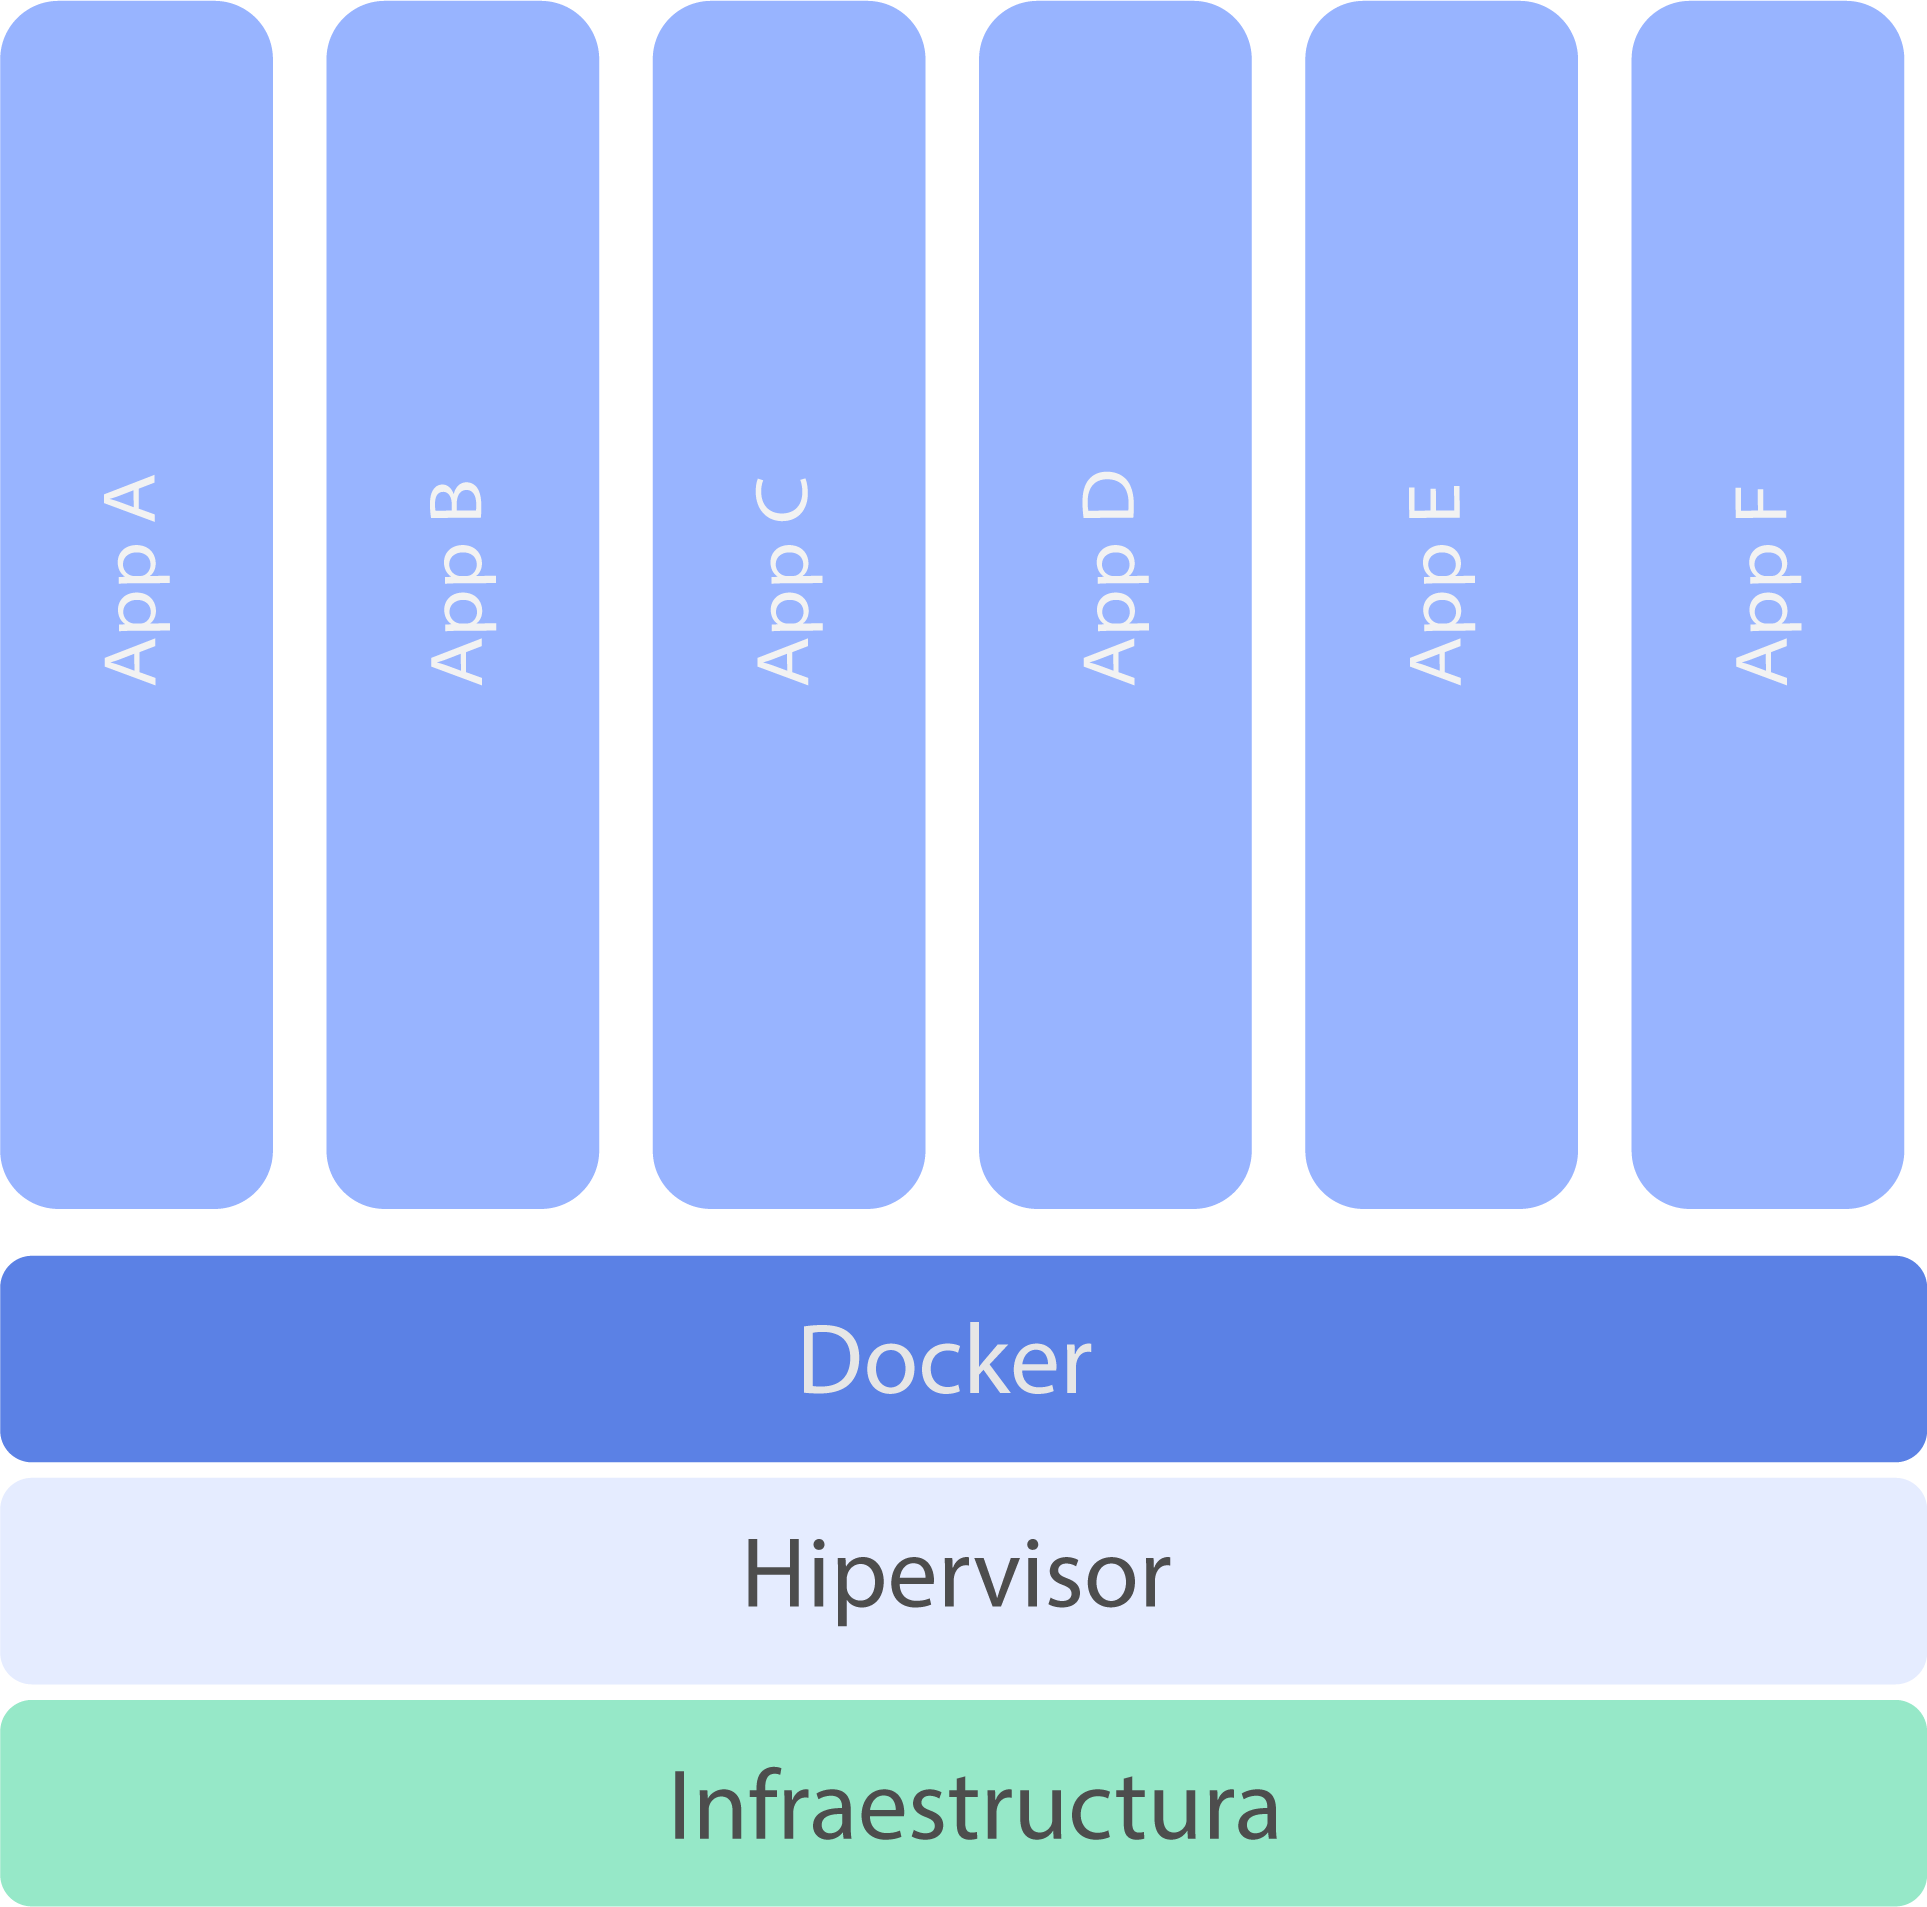
\includegraphics[scale=0.7]{images/containers.png}
  \captionof{figure}{Contenedor vs VM}
  \label{fig:contvm}
\end{figure}

\break

Los contenedores son una abstracción de la capa de aplicación que empaqueta el código y las dependencias juntos. Múltiples contenedores pueden correr en la misma máquina compartiendo el kernel del sistema operativo junto con otros contenedores, todos corriendo de forma aislada. Los contenedores ocupan menos espacio que las VMs.

\begin{figure}[h!]
  \centering
    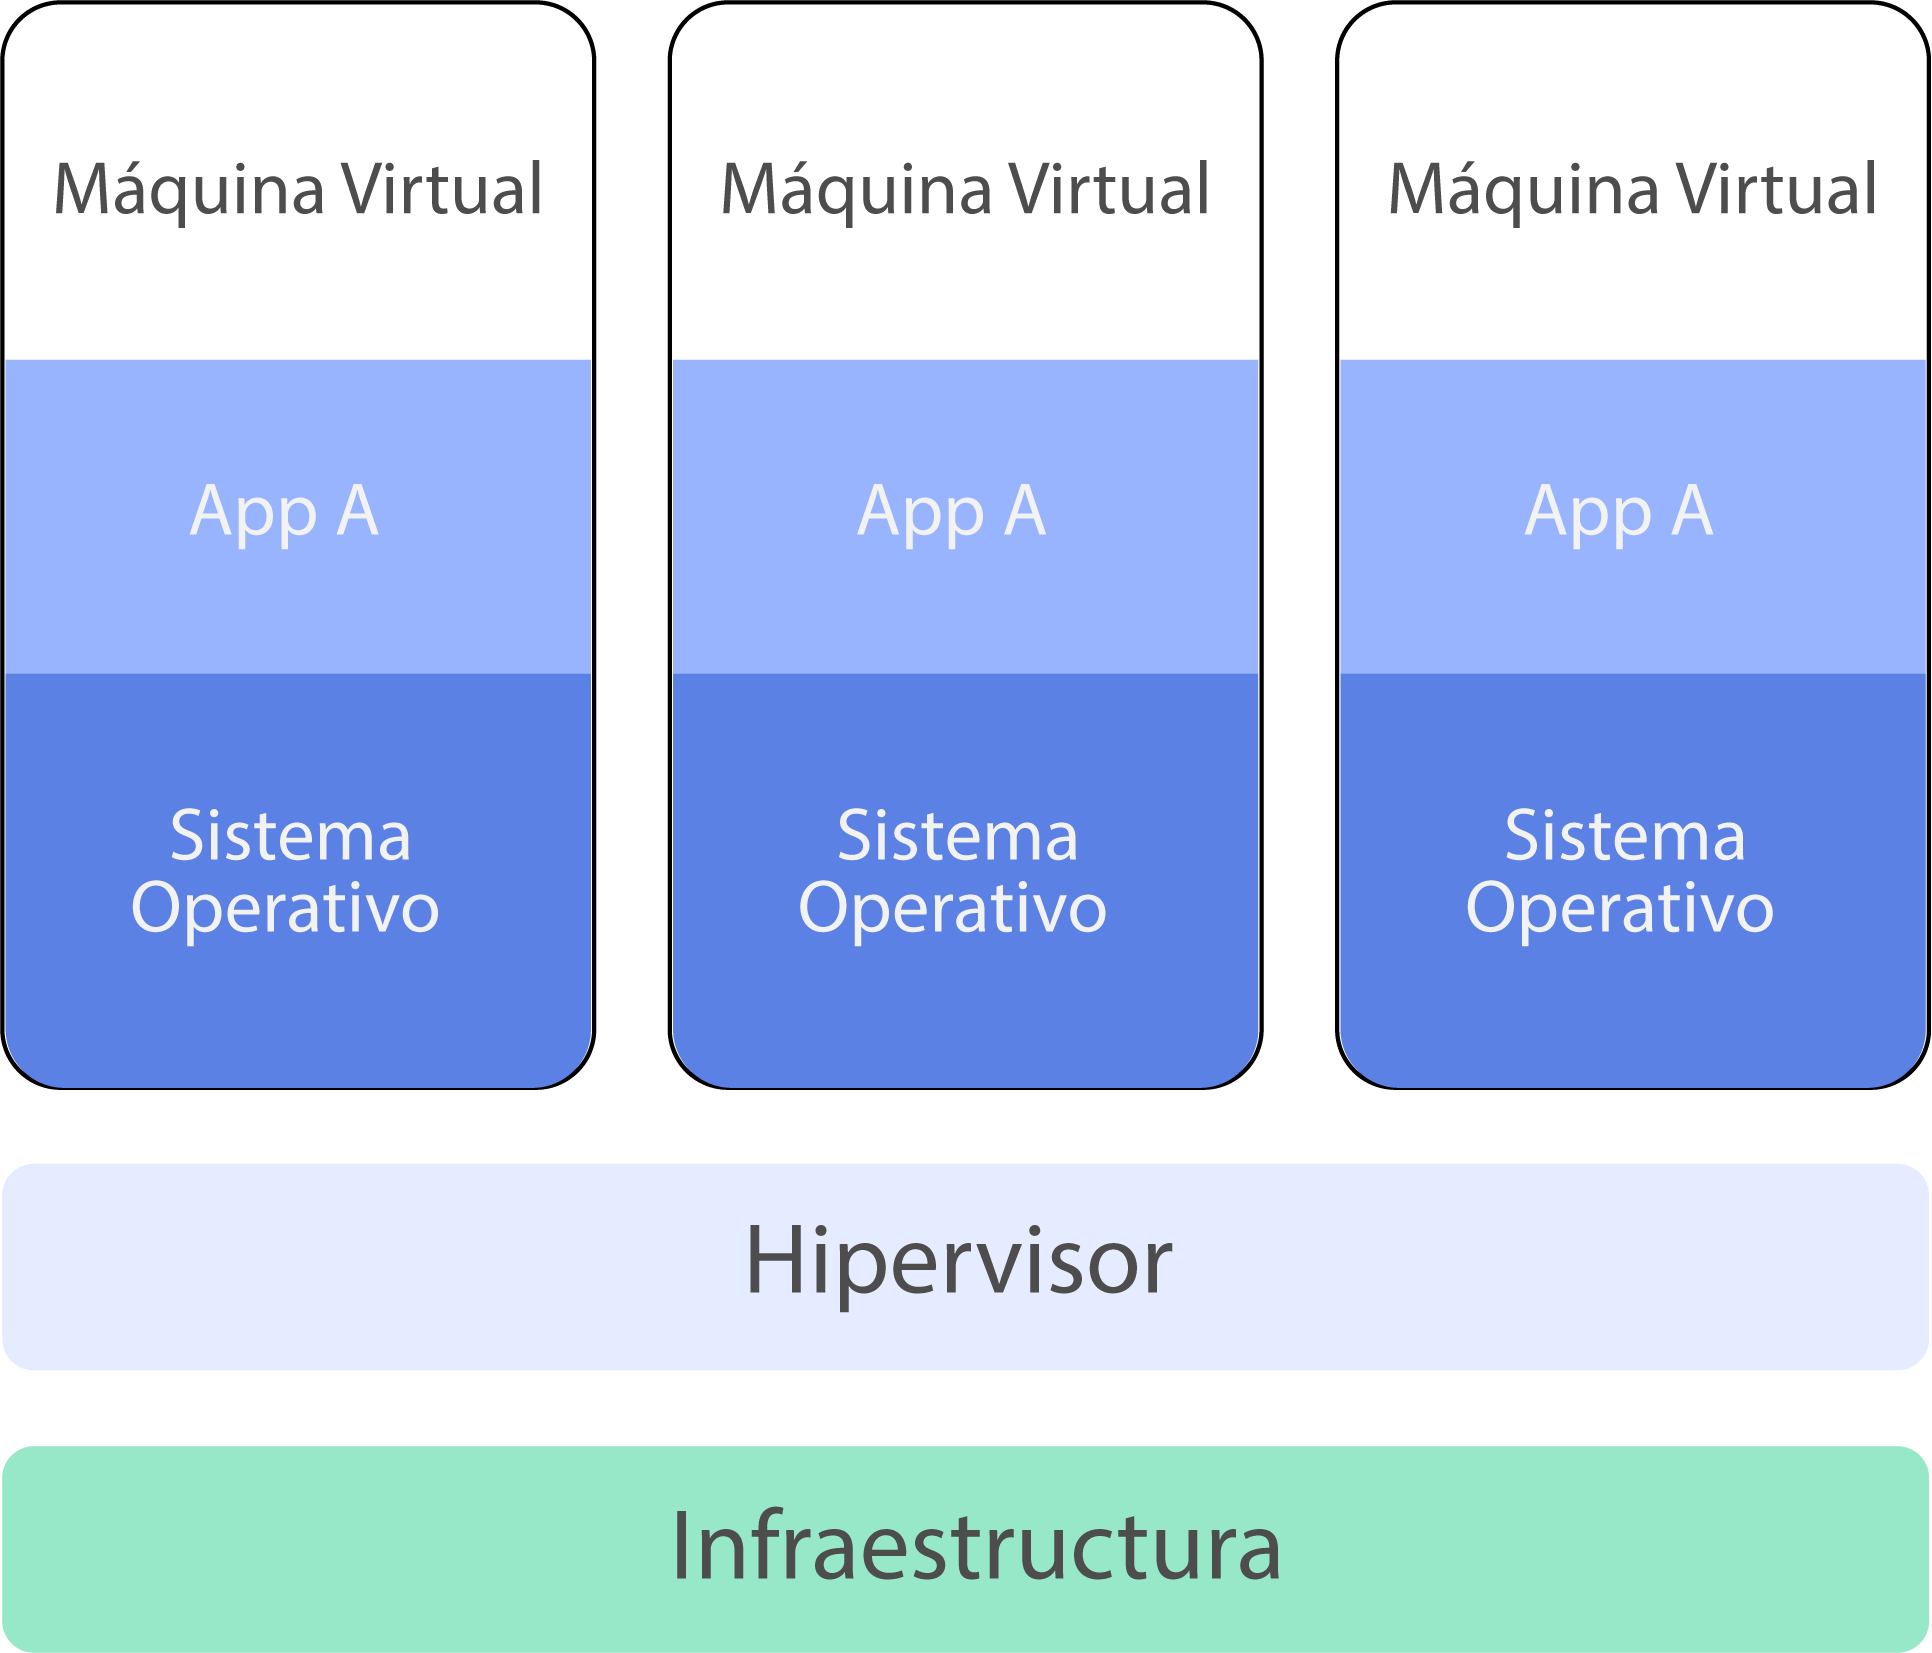
\includegraphics[scale=0.7]{images/vms.png}
  \captionof{figure}{Máquinas virtuales}
  \label{fig:vm}
\end{figure}

\break

Las máquinas virtuales (VMs) son una abstracción del hardware físico, transformando un servidor en múltiples servidores. El hypervisor permite que múltiples VMs corran en una misma máquina. Cada VM incluye una copia de un sistema operativo, la aplicación, los binarios y librerías, ocupando decenas de GBs.


\subsection[Docker Compose]{Docker Compose}

Docker Compose es una herramienta que permite correr un sistema formado por múltiples contenedores. Para ello, se debe crear un archivo .yml en el que se definan los servicios con los que va a contar la aplicación. Cada servicio estará formado por un contenedor corriendo una imágen de Docker. 
Para cada servicio pueden definirse nombres, puertos expuestos, conexiones de red, etc. Luego, con los siguientes comandos se puede operar con el sistema.

\section[Nginx]{Nginx}

Nginx es uno de los web servers más populares. Sirve tráfico HTTP y HTTPS, proxys a Python, NodeJS, corre software como balanceador de carga, http cache, SSL, etc.
Nginx es una pieza de software extremadamente modular. Muchas de las funcionalidades que trae por defecto, son en realidad módulos que se pueden activa y desactivar en cualquier momento. Una de las ventajas es que se puede decidir qué módulos se quiere utilizar, y cuales no.
Una de las funcionalidades más importantes para el desarrollo de microservicios es el proxy reverso.

\subsection[Forward proxy vs reverse proxy]{Forward proxy vs reverse proxy}

Una de las razones más populares para usar nginx es para que sirva aplicaciones dinámicas escritas en Python, NodeJS, Ruby, y muchas otras.
A diferencia de Apache, nginx no tiene la habilidad de embeber un intérprete al webserver, como hace Apache con mod\_php. En su lugar, nginx toma un enfoque mucho mas liviano. Es simplemente un webserver y su tarea principal es correr una aplicación web delegandolo a un server y proxies separados.

\subsection[Forward Proxy]{Forward Proxy}

Se le llama *forward proxy* a la configuración por defecto que se encuentra en todas las conexiones salientes de internet. Se ve algo asi:

\begin{figure}[h!]
  \centering
    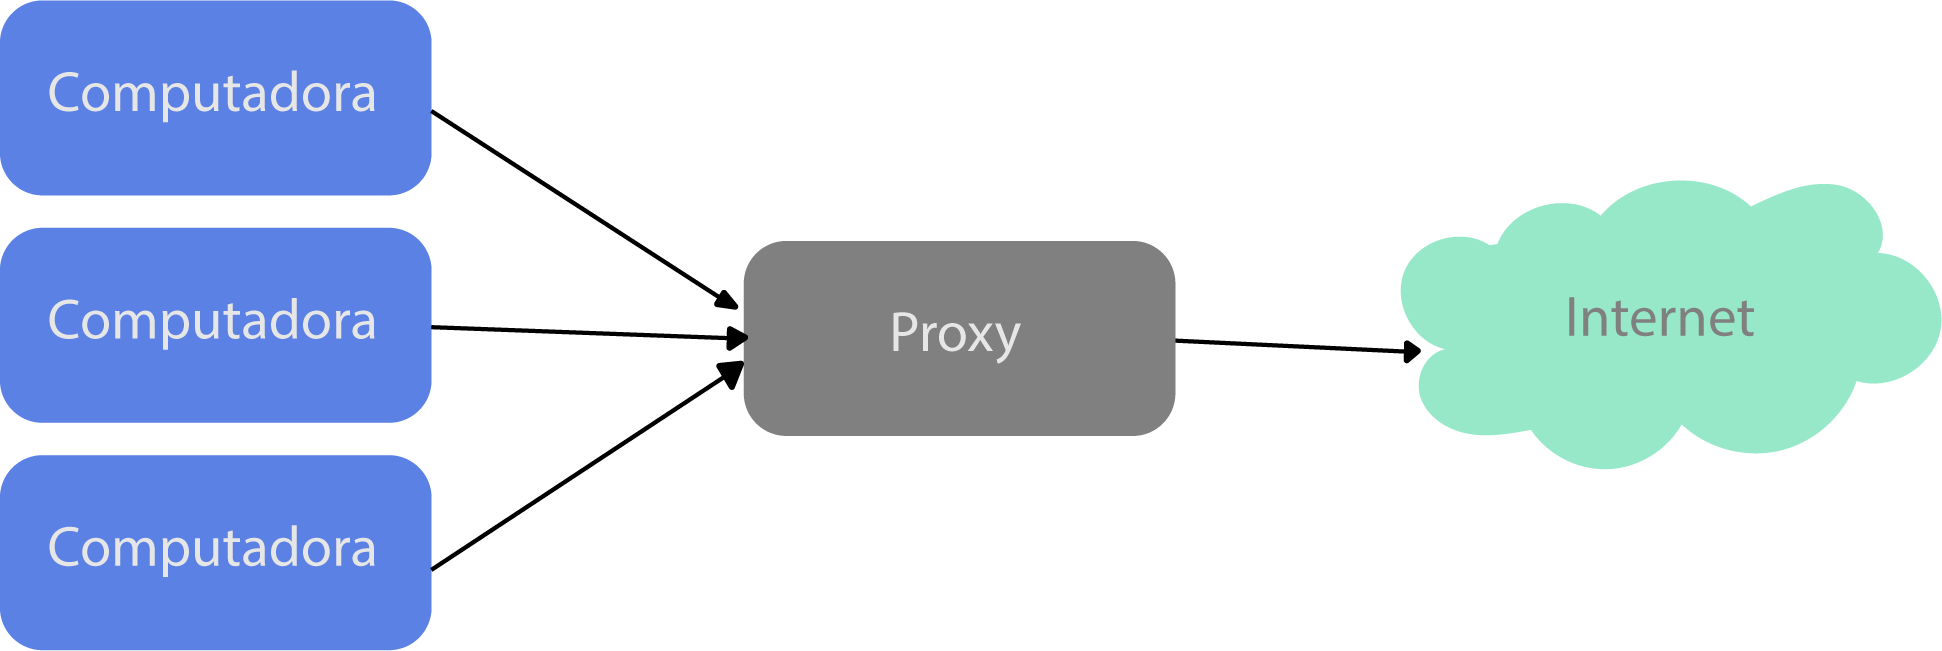
\includegraphics[scale=0.7]{images/forward-proxy.png}
  \captionof{figure}{Funcionamiento de Forward Proxy}
  \label{fig:forwardproxy}
\end{figure}

Las conexiones salientes de una computadora son capturadas por el *forward proxy* y reenviadas a Internet. Para Internet, todas las computadoras aparecen como si vinieran del mismo lugar- el *forward proxy*.


\subsection[Reverse Proxy]{Reverse Proxy}

Se le llama *reverse proxy* a lo opuesto de *forward proxy*, y es una configuración muy común para servir aplicaciones web dinámicas y para balance de carga.

\begin{figure}[h!]
  \centering
    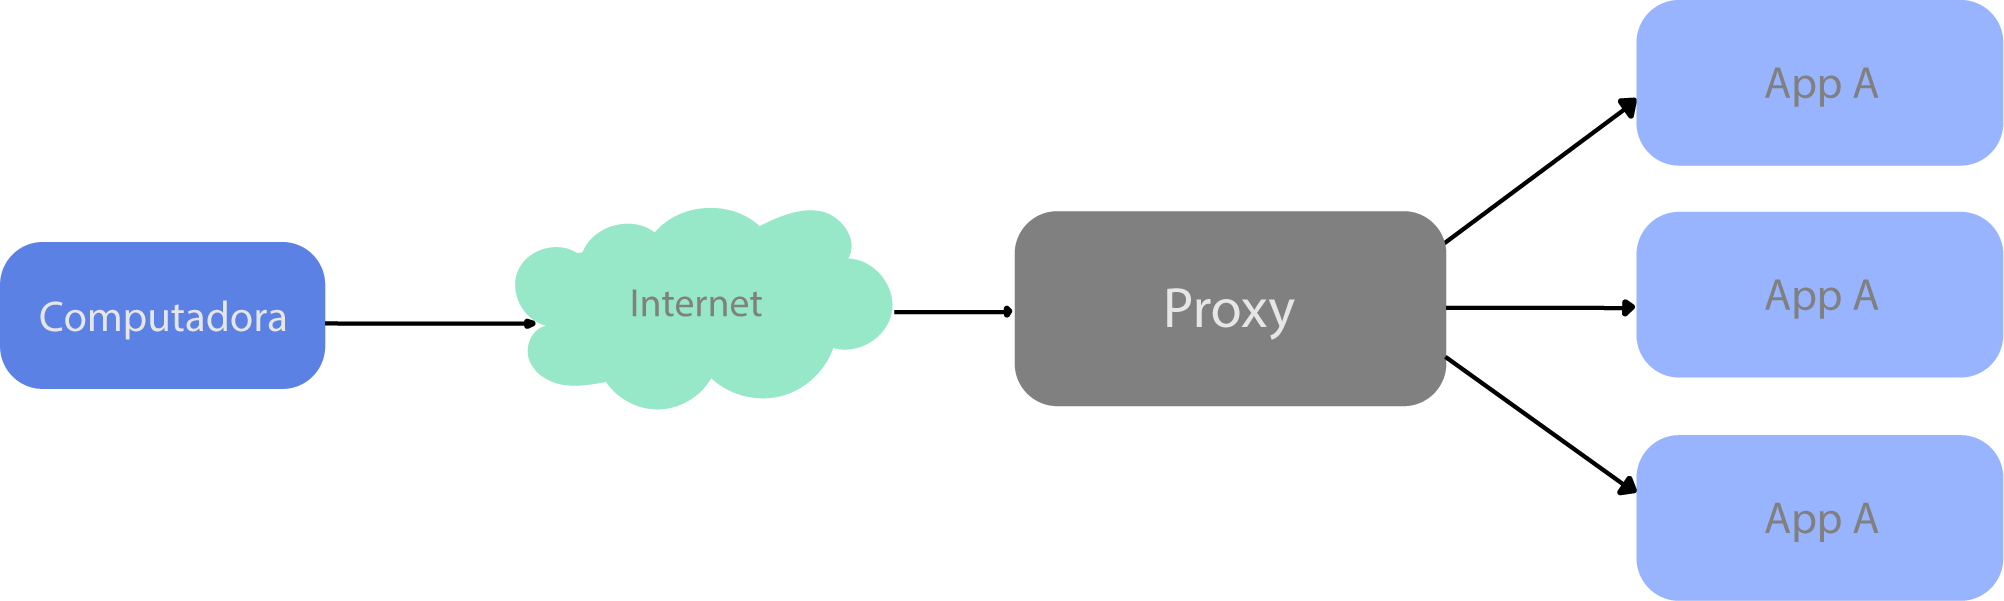
\includegraphics[scale=0.7]{images/reverse-proxy.png}
  \captionof{figure}{Funcionamiento de Reverse Proxy}
  \label{fig:reverseproxy}
\end{figure}

En este ejemplo, el *reverse proxy* hace de multiplexor para muchas conexiones de internet, a una aplicación dinámica. El *reverse proxy* mira el request, y lo reenvia a la aplicación.

\subsection[Balance de carga]{Balance de carga}

Una de las formas mas comunes de escalar una aplicación web es usar *balance de carga*. La idea detrás de esto, es distribuir la carga, o tráfico web, a través de diferentes *application servers*.
El funcionamiento normal de una sola aplicación con nginx es que los visitantes ingresan el nombre de dominio y son ruteados directamente al servidor donde nginx está sirviendo la *única* aplicación. El problema de esto es que cuando se tienen miles de conexiones visitando la aplicación, es probable que un solo servidor no pueda manejarlo. 
Ahi es cuando juega un papel importante el balanceador de carga, que recibe todo el tráfico ingresante y lo distribuye a través de un conjunto de servidores de aplicación.
Existen distintos tipos de balanceos de carga: por software y por hardware. Nginx tiene la habilidad de correr como un balanceador de carga de software, usando el módulo http_proxy.

El balance de carga es en definitiva un *reverse proxy*, con tres diferencias fundamentales: 
\begin{outline}
\1 Los balanceadores de carga reenvian el trafico a traves de varios *backends*, mientras que un reverse proxy tradicional lo hace hacia uno solo.
\1 Los balanceadores de carga usualmente operan en la capa 7 (HTTP) o en la capa 4 (TCP) del modelo OSI, cuando típicamente sólo operariamos en la capa 7 usando un *reverse proxy* de aplicaciones modernas.
\1 La escala es crítica para los balanceadores de carga: en sitios ocupados, pueden ver 20 veces la cantidad de tráfico que recibe un servidor de aplicación. Por ejemplo, un servidor de aplicaciones potente solo necesitará manejar entre 100 y 200 solicitudes por segundo, mientras que un balanceador de carga puede recibir más de 10,000 solicitudes por segundo.
\end{outline}